\chapter{Erstes Kapitel}
\label{kap:eins}
Dies ist eine Vorlage für wissenschaftliche Arbeiten an der FHGR nach \textcite{stepanenko_leitfaden_2023}\footnote{Quelle aus dem Intranet (nicht öffentlich zugänglich) von FHGR}. Nachfolgend einige Tipps und Funktionen, welche in der Vorlage enthalten sind.

\section{Glossar und Abkürzungen}
Mit den Befehlen \lstinline|acrlong{zb}|, \lstinline|acrshort{zb}| oder \lstinline|acrfull{zb}| ist das Ausgeben der im Dokument \lstinline{content/00_assets/01_Vorspann/01.4_abkuerzungsverzeichnis_glossar.tex} Einträgen möglich: \acrshort{zb}, \acrshort{zb}, \acrfull{zb}.

\section{Zitieren}
Für das Setzen von Anführungszeichen stehen verschiedene Möglichkeiten zur Verfügung. Mittels \lstinline|\enquote{...}| können Texte in Anführungszeichen gesetzt werden. Zum Beispiel: \\\lstinline|\enquote{Ein wörtliches Zitat}| ergibt \enquote{Das ist ein wörtliches Zitat}. Guillemets können auch mittels \lstinline{"<} und \lstinline{">} gesetzt werden. Als Beispiel \lstinline{"<Ein wörtliches Zitat">} ergibt "<Ein wörtliches Zitat">. Ein Blockzitat kann mittels des Befehls \lstinline|\blockquote{...}| erstellt werden. Die Ausgabe eines Blockzitats sieht folgendermassen aus:

\blockquote{Blockzitate sind wörtliche Zitate von 40 Wörtern oder mehr; sie werden als eigener Absatz ohne Anführungszeichen angeführt. Ein Blockzitat beginnt stets in einer neuen Zeile, wird zur Gänze (also jede Zeile) 1,3 cm oder fünf Leerschritte eingerückt und mit zweizeiligem Abstand geschrieben. Absätze innerhalb eines Blockzitates werden vom neuen Rand des Blockzitates eingerückt. \par Blockzitate werden nicht in Anführungszeichen gesetzt, darin aufscheinende Zitate werden in doppelten Anführungszeichen wiedergegeben. \par Die Quellenangabe am Ende eines Blockzitates steht nach dem letzten schlie"senden Punkt des Zitates in Klammern gesetzt, danach folgt kein weiterer Punkt.\\
\parencite[S. 111]{psychologie_richtlinien_2016}}
\noindent
Weitere Möglichkeiten können der Dokumentation\footnote{http://mirrors.ctan.org/macros/latex/contrib/csquotes/csquotes.pdf} zum \texttt{csquotes} Paket entnommen werden.
\newpage
Für die Quellverwaltung wird das Paket \texttt{biblatex} mit dem APA Zitationsstil verwendet. Die umfangreiche Dokumentation\footnote{https://mirror.metanet.ch/tex-archive/info/translations/biblatex/de/biblatex-de-Benutzerhandbuch.pdf} bietet einen Überblick aller möglichen Befehle. Voraussetzung ist, dass die Quellen erst im BibLaTeX Format unter \lstinline{content/00_assets/quellen.bib} abgelegt sind (z. B. via Zotero / Mendely\footnote{https://www.overleaf.com/learn/how-to/How\_to\_link\_your\_Overleaf\_account\_to\_Mendeley\_and\_Zotero} oder als Datei). Nachfolgend einige Beispiele mit den üblichsten Befehlen:\\
\\
\lstinline|\textcite{diani_black_2016}| gibt als Ausgabe:
\textcite{diani_black_2016}\\
\lstinline|\parencite{diani_black_2016}| gibt als Ausgabe:
\parencite{diani_black_2016}\\
\lstinline|\parencites[S. 10]{diani_black_2016}[S. 20]{stepanenko_leitfaden_2023}| gibt als Ausgabe:
\parencites[S. 10]{diani_black_2016}[S. 20]{stepanenko_leitfaden_2023}\\
\\
Zusätzlich stehen die folgenden eigens im Template definierten Befehle zur Verfügung, bei welchen die im \lstinline{content/01_vorspann/01.4_abkuerzungsverzeichnis_glossar.tex} definierten Abkürzungen verwendet werden können:\\
\\
\lstinline|parenciteabbr{org_2022}{orln}| gibt als Ausgabe: \parenciteabbr{org_2022}{orln}\\
\\
\lstinline|textciteabbr{org_2022}{orln}| gibt als Ausgabe: 
\textciteabbr{org_2022}{orln}\\

\chapter{Ein Bild}
\begin{figure}[H]
    \caption{Überschrift Abbildung 1}
    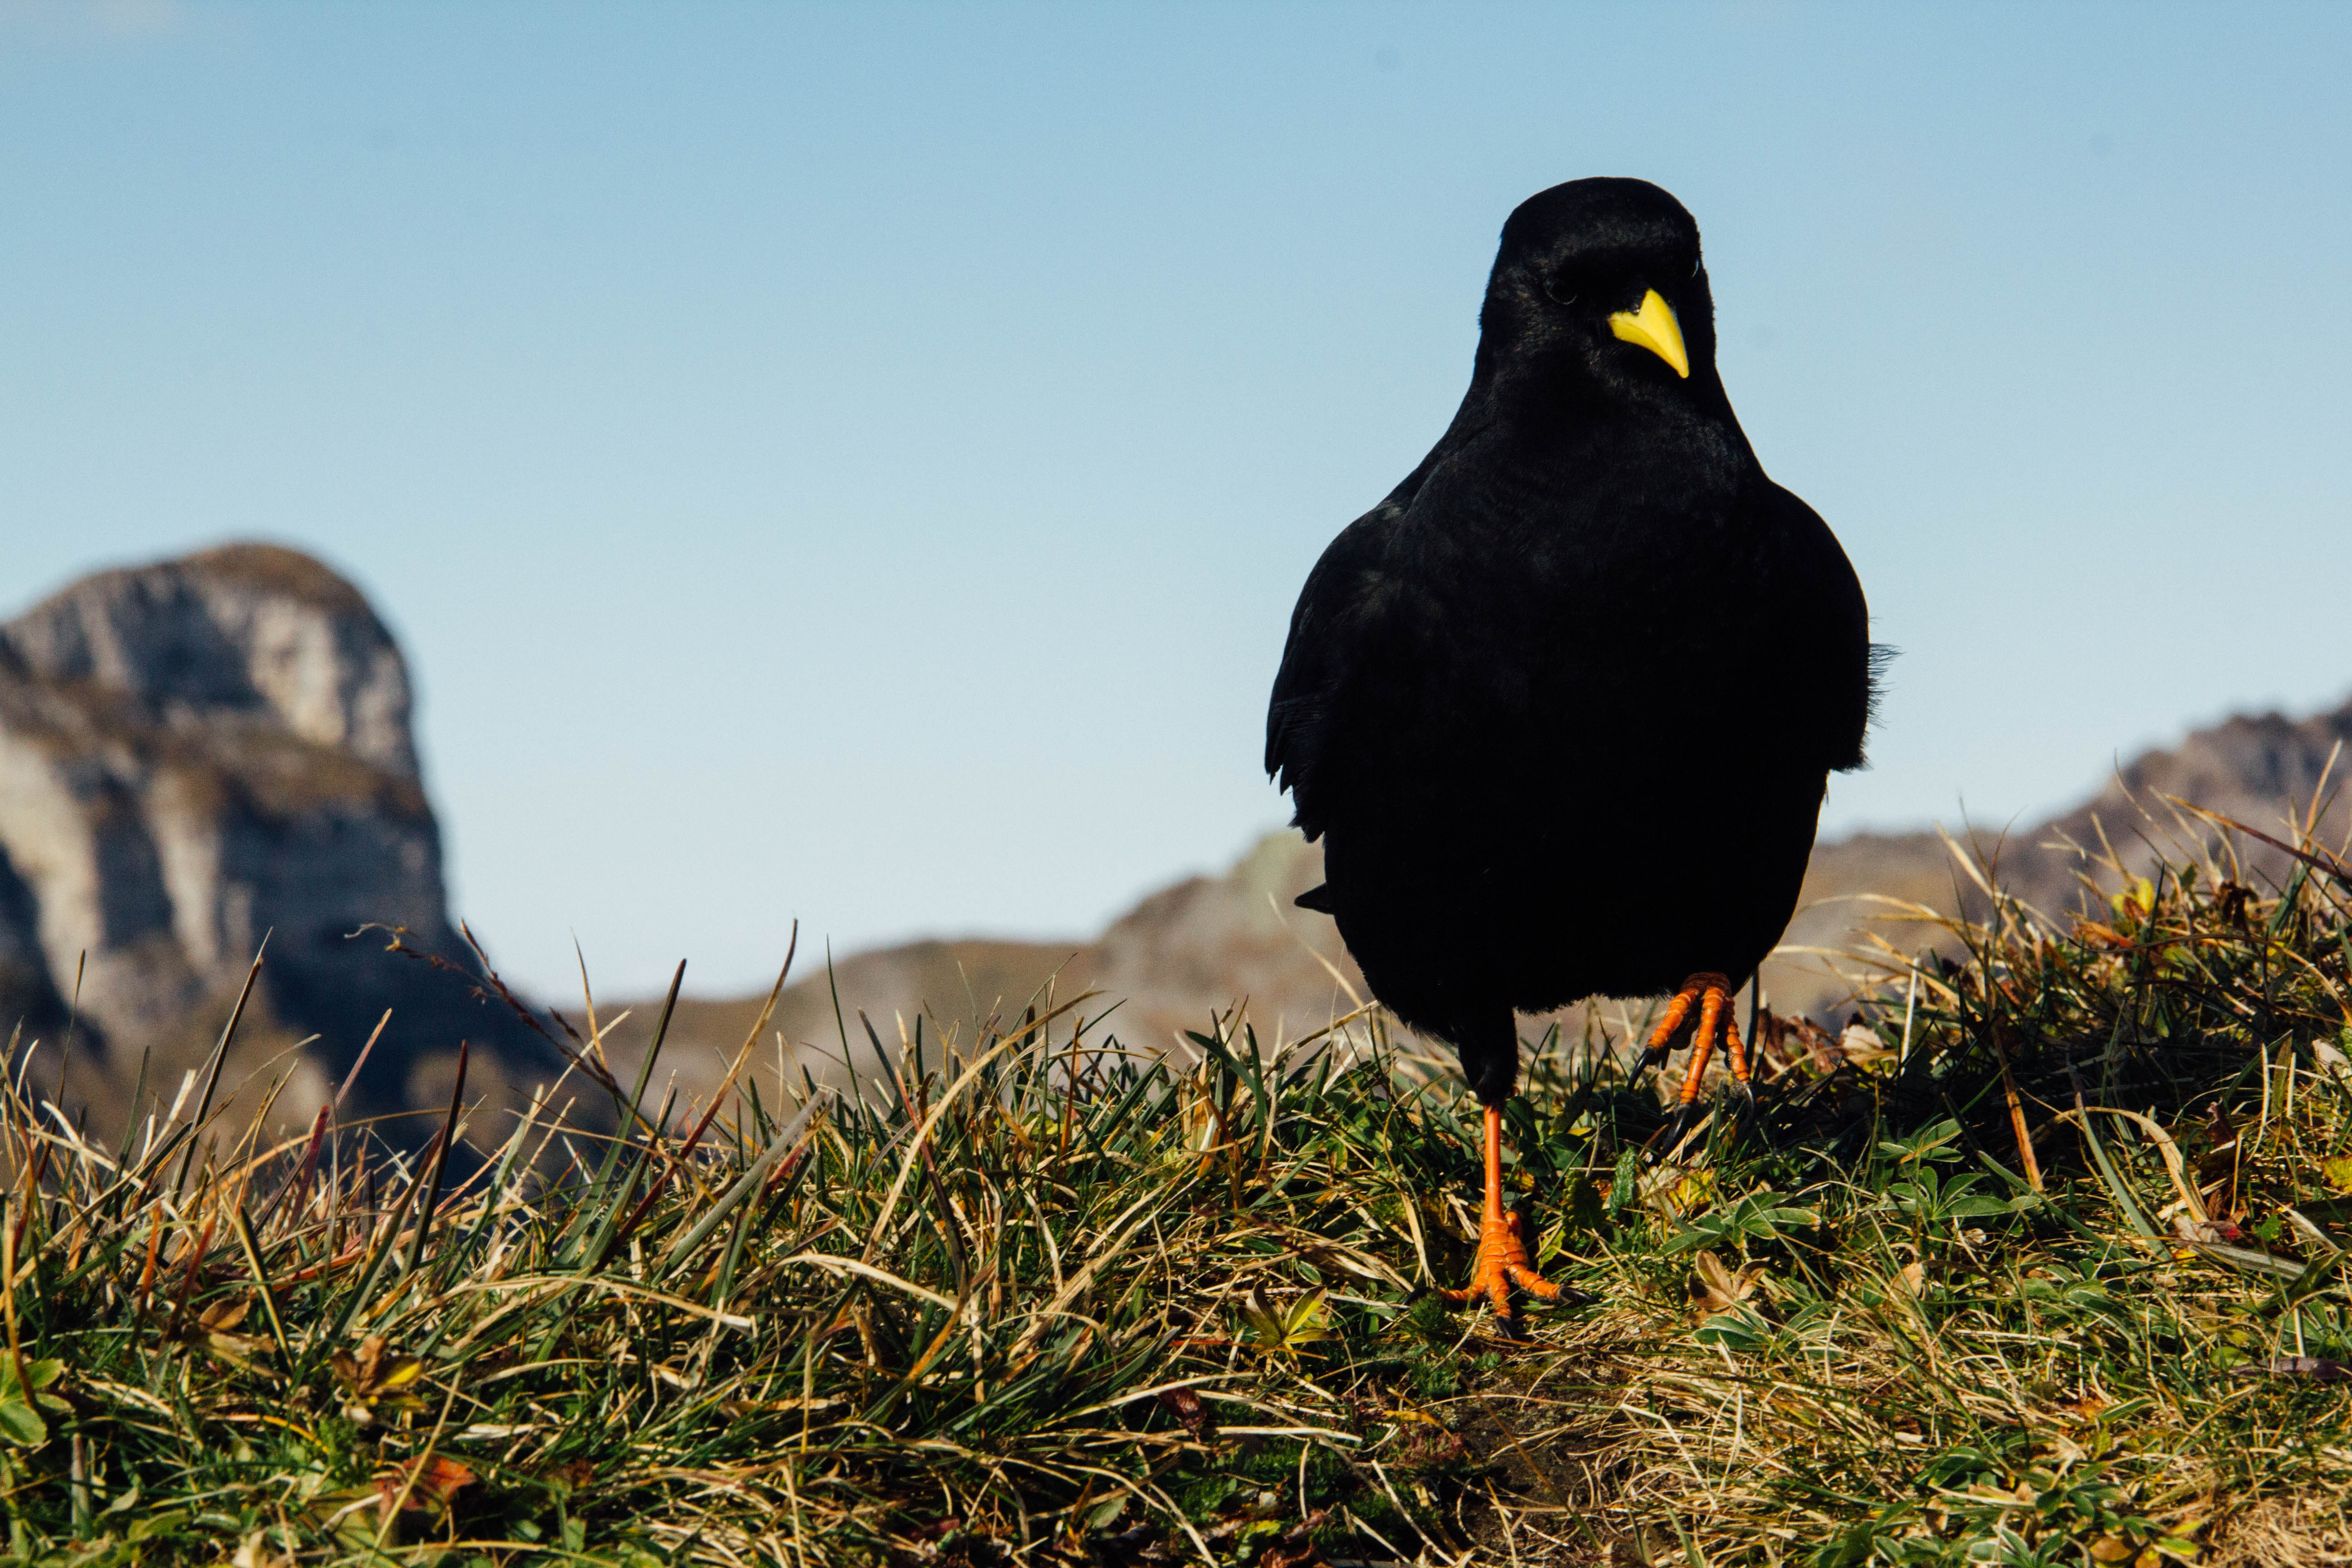
\includegraphics[width=\textwidth]{alpendohle.jpg}
    \note{\textcite[Abs. 1]{diani_black_2016}}
    \label{fig:alpendohle}
\end{figure}

\chapter{Tabelle}
Im folgenden (Tabelle \ref{tab:tabelle}) ist ein Beispiel einer Tabelle:
\begin{table}[ht]
    \caption{Überschrift Tabelle 1}
    \begin{tabularx}{\textwidth} {
        >{\raggedright\arraybackslash}X 
        >{\raggedleft\arraybackslash}X 
        >{\raggedleft\arraybackslash}X}
            \hline
            \multicolumn{3}{c}{\textbf{Beispieltabelle}}\\
            \hline
            \textbf{Linksbündig} & \textbf{Rechtsbündig} & \textbf{Rechtsbündig}\\
            \hline
            Lorem & N/A & N/A\\
            Ipsum & 1 499 & 8 512\\
            Dolor & 297 & N/A\\
            Sit & 1 053 & N/A\\
            \hline
            \textbf{Total} & 2 849 & 8 512\\
            \hline
    \end{tabularx}
    \medbreak
    \note{\textcite[Abs. 1]{diani_black_2016}}
    \label{tab:tabelle}
\end{table}

\chapter{Programmcode}
Programmcode ist immer öfter Bestandteil von Studienarbeiten. Die \textcite{American_Psychological_Association_2022} schreibt zur Formatierung von Passagen mit Porgrammcode: "<To present computer code, use a monospace font such as 10-point Lucida Console or 10-point Courier New">. Im Fliesstext könnte dies folgendermassen aussehen: Die Funktion \lstinline{print()} in der Programmiersprache Python wird meist dazu benutzt, Text auf dem Bildschirm auszugeben. Das folgende Beispiel \ref{code:hello} gibt die Zeichenkette "<Hello World"> aus.
\begin{lstlisting}[language=Python,caption=Überschrift Programmcode,label=code:hello] 
# hello_world.py
print("Hello World!")
\end{lstlisting}
\medbreak
\noindent
Weitere Konfigurationsmöglichkeiten für die Darstellung von Programmcode können der Dokumentation\footnote{http://texdoc.net/texmf-dist/doc/latex/listings/listings.pdf} des \texttt{lstlisting} Pakets entnommen werden. 